
%(BEGIN_QUESTION)
% Copyright 2010, Tony R. Kuphaldt, released under the Creative Commons Attribution License (v 1.0)
% This means you may do almost anything with this work of mine, so long as you give me proper credit

Calculate the appropriate LRV and URV pressures for this hydrostatic level measurement system, assuming the process liquid has a weight density of 44 pounds per cubic foot at a temperature of 23 degrees Celsius, and that the ``wet leg'' compensating impulse line is filled with a glycerin/water mix (S.G. = 1.13).  Assume a static vessel pressure of 126 PSI:

$$\includegraphics[width=15.5cm]{i03747x01.eps}$$

Express your answers in units of {\it inches water column} ("W.C. or "H$_{2}$O).

\vskip 20pt \vbox{\hrule \hbox{\strut \vrule{} {\bf Suggestions for Socratic discussion} \vrule} \hrule}

\begin{itemize}
\item{} As liquid level increases in this vessel, will the transmitter's signal increase or decrease (i.e. is this level transmitter {\it direct} or {\it reverse} acting?
\item{} If the process liquid heats up and becomes less dense (but the actual level remains the same), will the transmitter's 4-20 mA signal increase, decrease, or remain the same?
\item{} If the wet leg is filled with pure glycerin instead of a glycerin/water mixture (but the process liquid level remains the same), will the transmitter's 4-20 mA signal increase, decrease, or remain the same?
\item{} How would this system respond if someone closed the upper nozzle block valve, isolating the compensating leg impulse line from the process vessel?
\item{} Describe a step-by-step procedure for re-filling the wet leg with glycerin, assuming a pressurized vessel.
\end{itemize}

\underbar{file i03747}
%(END_QUESTION)





%(BEGIN_ANSWER)

LRV = +173.7 "H$_{2}$O \hskip 50pt URV = +94.76 "H$_{2}$O

\vskip 10pt

The temperature and static pressure values are extraneous information, included for the purpose of challenging students to identify whether or not information is relevant to solving a particular problem.

%(END_ANSWER)





%(BEGIN_NOTES)

Hydrostatic pressure on ``H'' side:

\vskip 10pt

(198 inches)(1.13) = 223.74 "WC

\vskip 20pt

Process liquid SG = 44/62.428 = 0.7048

\vskip 10pt

Hydrostatic pressure on ``L'' side at LRV = (71 inches)(0.7048) = 50.04 "WC

\vskip 10pt

Hydrostatic pressure on ``L'' side at URV = (183 inches)(0.7048) = 128.98 "WC

\vskip 20pt

LRV = 223.74 $-$ 50.04 = {\bf 173.70 "WC}

\vskip 10pt

URV = 223.74 $-$ 128.98 = {\bf 94.76 "WC}

%INDEX% Measurement, level: hydrostatic pressure

%(END_NOTES)

